\begin{example2}[\quad \large Fordulatszám és pozíció érzékelés 6.]

Rajzolja fel 1ms-ra az inkrementális fordulatszámadó A és B jeleinek időfüggvényét számszerűen is helyes, ha D=1000 és n=60/perc! Mekorra sebességgel halad a robot, ha a kerékátmérő 10 cm?

\end{example2}

Először is nézzük a paramétereket: \\

$D\;=\;1000$, azaz 1000 osztás található a tárcsa kerületén. \\

Inneen könnyedén meghatáozhatjuk az egyes impulzusok periódusidejét, aminek segítségével pedig elkészíthetjük az ábrát.

\begin{equation}
\begin{aligned}{}
    n\;&=\;60\; / \; min \; = \; 1/s \\
    T\; &= \; \frac{n}{D}\; = \; \frac{\frac{1}{s}}{1000}\;=\;1\;ms \\
\end{aligned}
\end{equation}

Az Inkrementális jeladó jelalakjai a követkeőképpen néznek ki:

\begin{figure}[h!]
    \centering
         \begin{subfigure}[b]{0.24\textwidth}
         \centering
         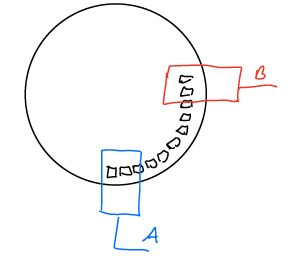
\includegraphics[width=\textwidth]{Figures//tmp/43_tarcsa.png}
         \caption{Inkrementális jeladó tárcsa}
         \label{fig:y equals x}
     \end{subfigure}
     \hfill
     \begin{subfigure}[b]{0.6\textwidth}
         \centering
         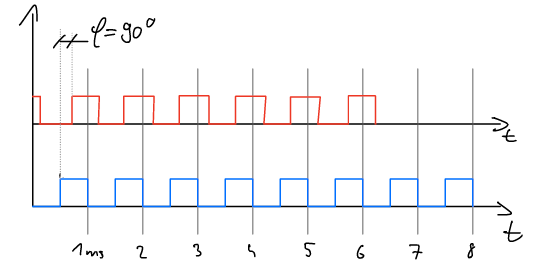
\includegraphics[width=\textwidth]{Figures//tmp/43_jelalak.png}
         \caption{A és B hullámformák}
         \label{fig:three sin x}
     \end{subfigure}
    \caption{Inkrementális jeladó}
    \label{fig:enter-label}
\end{figure}

Utolsó lépésben határozzuk meg a robot sebességét:

\begin{equation}
\begin{aligned}{}
    K\;&=\; d \cdot \pi \approx \; 0,314\;m \\
    v\; &= \; K \cdot n = 0,314\;m \cdot \sfrac{1}{s} = \underline{0,314 \; \sfrac{m}{s}}\\
\end{aligned}
\end{equation}



